\documentclass[11pt,a4paper]{scrartcl}
\typearea{12}
\usepackage{graphicx}
\usepackage{pstricks}
\usepackage{amsmath}
\begin{document}


\section*{An introduction to programming}

To save time learning syntax we are going to look at a block
programming language where the commands appear as block. When you get
used to a programming language typing is, of course, quicker than
moving blocks around, but block programming languages are very
convenient; this programming environment is hosted online which is
even more convenient since it means we don't have to install
anything. The site an be found at \texttt{snap.berkeley.edu}.

Here is a simple programme for drawing a square; we will start with
this and try to make more complicated drawings.
\begin{center}
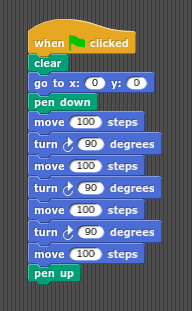
\includegraphics{basic_square.png}
\end{center}
Enter this and make sure it draws a square! One thing about this
program is that after it draws the square the arrow ends up pointing a
different direction to the direction it started in; can you fix this?

Now, the annoying thing about this programme is having to move over
the same two commands again and again; this isn't just a problem
because it is boring, it also disguises the main point of the program,
doing the same thing four times. Programmes are best when they are easy to interpret, so here we can make the programme simpler using a repeat:
\begin{center}

\includegraphics{repeat.png}
\end{center}
Can you use that to make the programme more succinct and readable? 

Now, look at this programme
\begin{center}
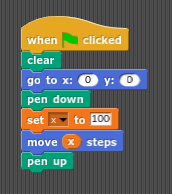
\includegraphics{variable.png}
\end{center}
Instead of writing directly that it is to go 100 steps and make a
\textsl{variable} called \texttt{x} and tell it to go \texttt{x}
steps. This is kind of pointless in this short program but we will see
soon how useful variables are. Do the same to your square programme!
You will need to click the \lq{}Make a variable\rq{} button to add a
variable; add it for all sprites, we'll only be using one sprite at a
time in this class.

This programme does something slighly more useful with a variable, it
goes forward a certain number steps, turns, then goes forward half as
far as before. Now, rather than having to put in the number of steps,
then work out half and put that in, it uses a variable for the number
of steps and another one to calculate half the number. 
\begin{center}
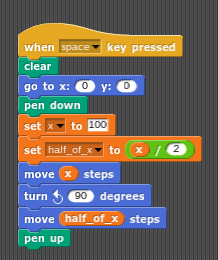
\includegraphics{line_half_line.png}
\end{center}
Try modifying your programme in a similar way so that it draws an
$n$-gon, notice that turning 90 degrees each time won't give an
$n$-gon, so you'll need to use a variable to instruct it to turn
\begin{equation}
\theta=\frac{360}{n}
\end{equation}
degrees each time.

In this programme the variable is changed in the \textsl{loop} so the
line is shorter each time:
\begin{center}
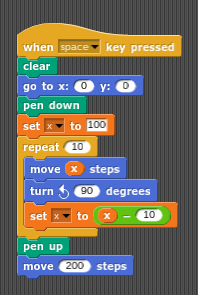
\includegraphics{spiral.png}
\end{center}
giving a spiral
\begin{center}

\includegraphics{spiral_pic.png}
\end{center}
Try modifying your programme in the same way so that you get smaller and smaller squares retreating into one corner, like this
\begin{center}
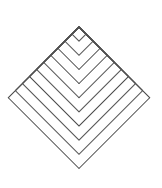
\includegraphics{repeat_squares_pic.png}
\end{center}
If you want to you can try playing with you program a bit to give other patterns, like this
\begin{center}
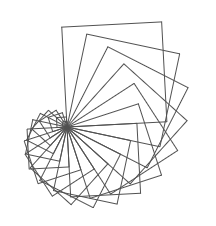
\includegraphics{squares_spiral_pic.png}
\end{center}

This next programme draws a star
\begin{center}
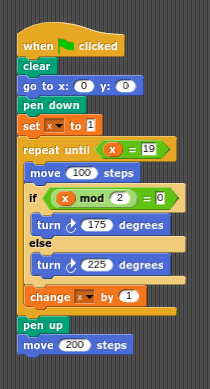
\includegraphics{star.png}
\end{center}
Input it and have a look and then try to understand it; it is intended
to illustrate the idea of conditional statements. There are two, first
the \textsl{repeat until}. This is similar to the repeat we used
before, but now, instead of repeating a set number of times, every
time it repeats it checks a condition, in this case \texttt{x=19}; if
the condition is true, it stops, otherwise it keeps repeating. In our
case one gets added to \texttt{x} each time, so eventually it will
stop. The other conditional statement is the \texttt{if . . . else}
statement. Because the star has two different angles we need two
different sorts of turns, in the if statement it does the first
possibility, turning 175 degrees if \texttt{x mod 2 = 0} and the other
otherwise. The meaning of \textsl{mod} is that it gies the remainder
after dividing, so \texttt{x mod 2} means the remainder after dividing
\texttt{x} by 2; this will be zero if \texttt{x} is even, odd
otherwise. 

You can mess with programme a bit, maybe changing the angles or putting the whole thing in a loop to give something like this
\begin{center}

\includegraphics{rotating_star_pic.png}
\end{center}
Finally have a look at this programme:
\begin{center}
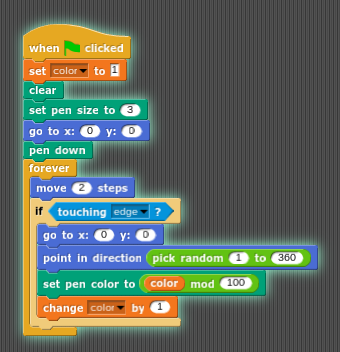
\includegraphics{center_rays.png}
\end{center}
It also has a conditional statement, but the condition is something outside the programme, in this case touching the edge.

\end{document}
